\documentclass[10 pt,usenames,dvipsnames, oneside]{article}
\usepackage{../../../modelo-ensino-medio}



\begin{document}

\begin{center}
  \begin{minipage}[l]{3cm}

\includegraphics[width=2cm]{logo}    
\end{minipage}\hfill
\begin{minipage}[r]{.8\textwidth}
 {\Large \scshape Atividade: Escolha da chave correta}  
\end{minipage}
\end{center}
\vspace{.2cm}

\ifdefined\prof
%Habilidades da BNCC
\begin{objetivos}
\item a
\end{objetivos}

%Caixa do Para o Professor
\begin{goals}
%Objetivos específicos
\begin{enumerate}
\item Estender a regra da multiplicação para o caso de mais de dois eventos.
\end{enumerate}

\end{goals}

\bigskip
\begin{center}
{\large \scshape Atividade}
\end{center}
\fi

Numa caixa há 5 chaves das quais apenas uma abre um cadeado.

\begin{figure}[H]
\centering
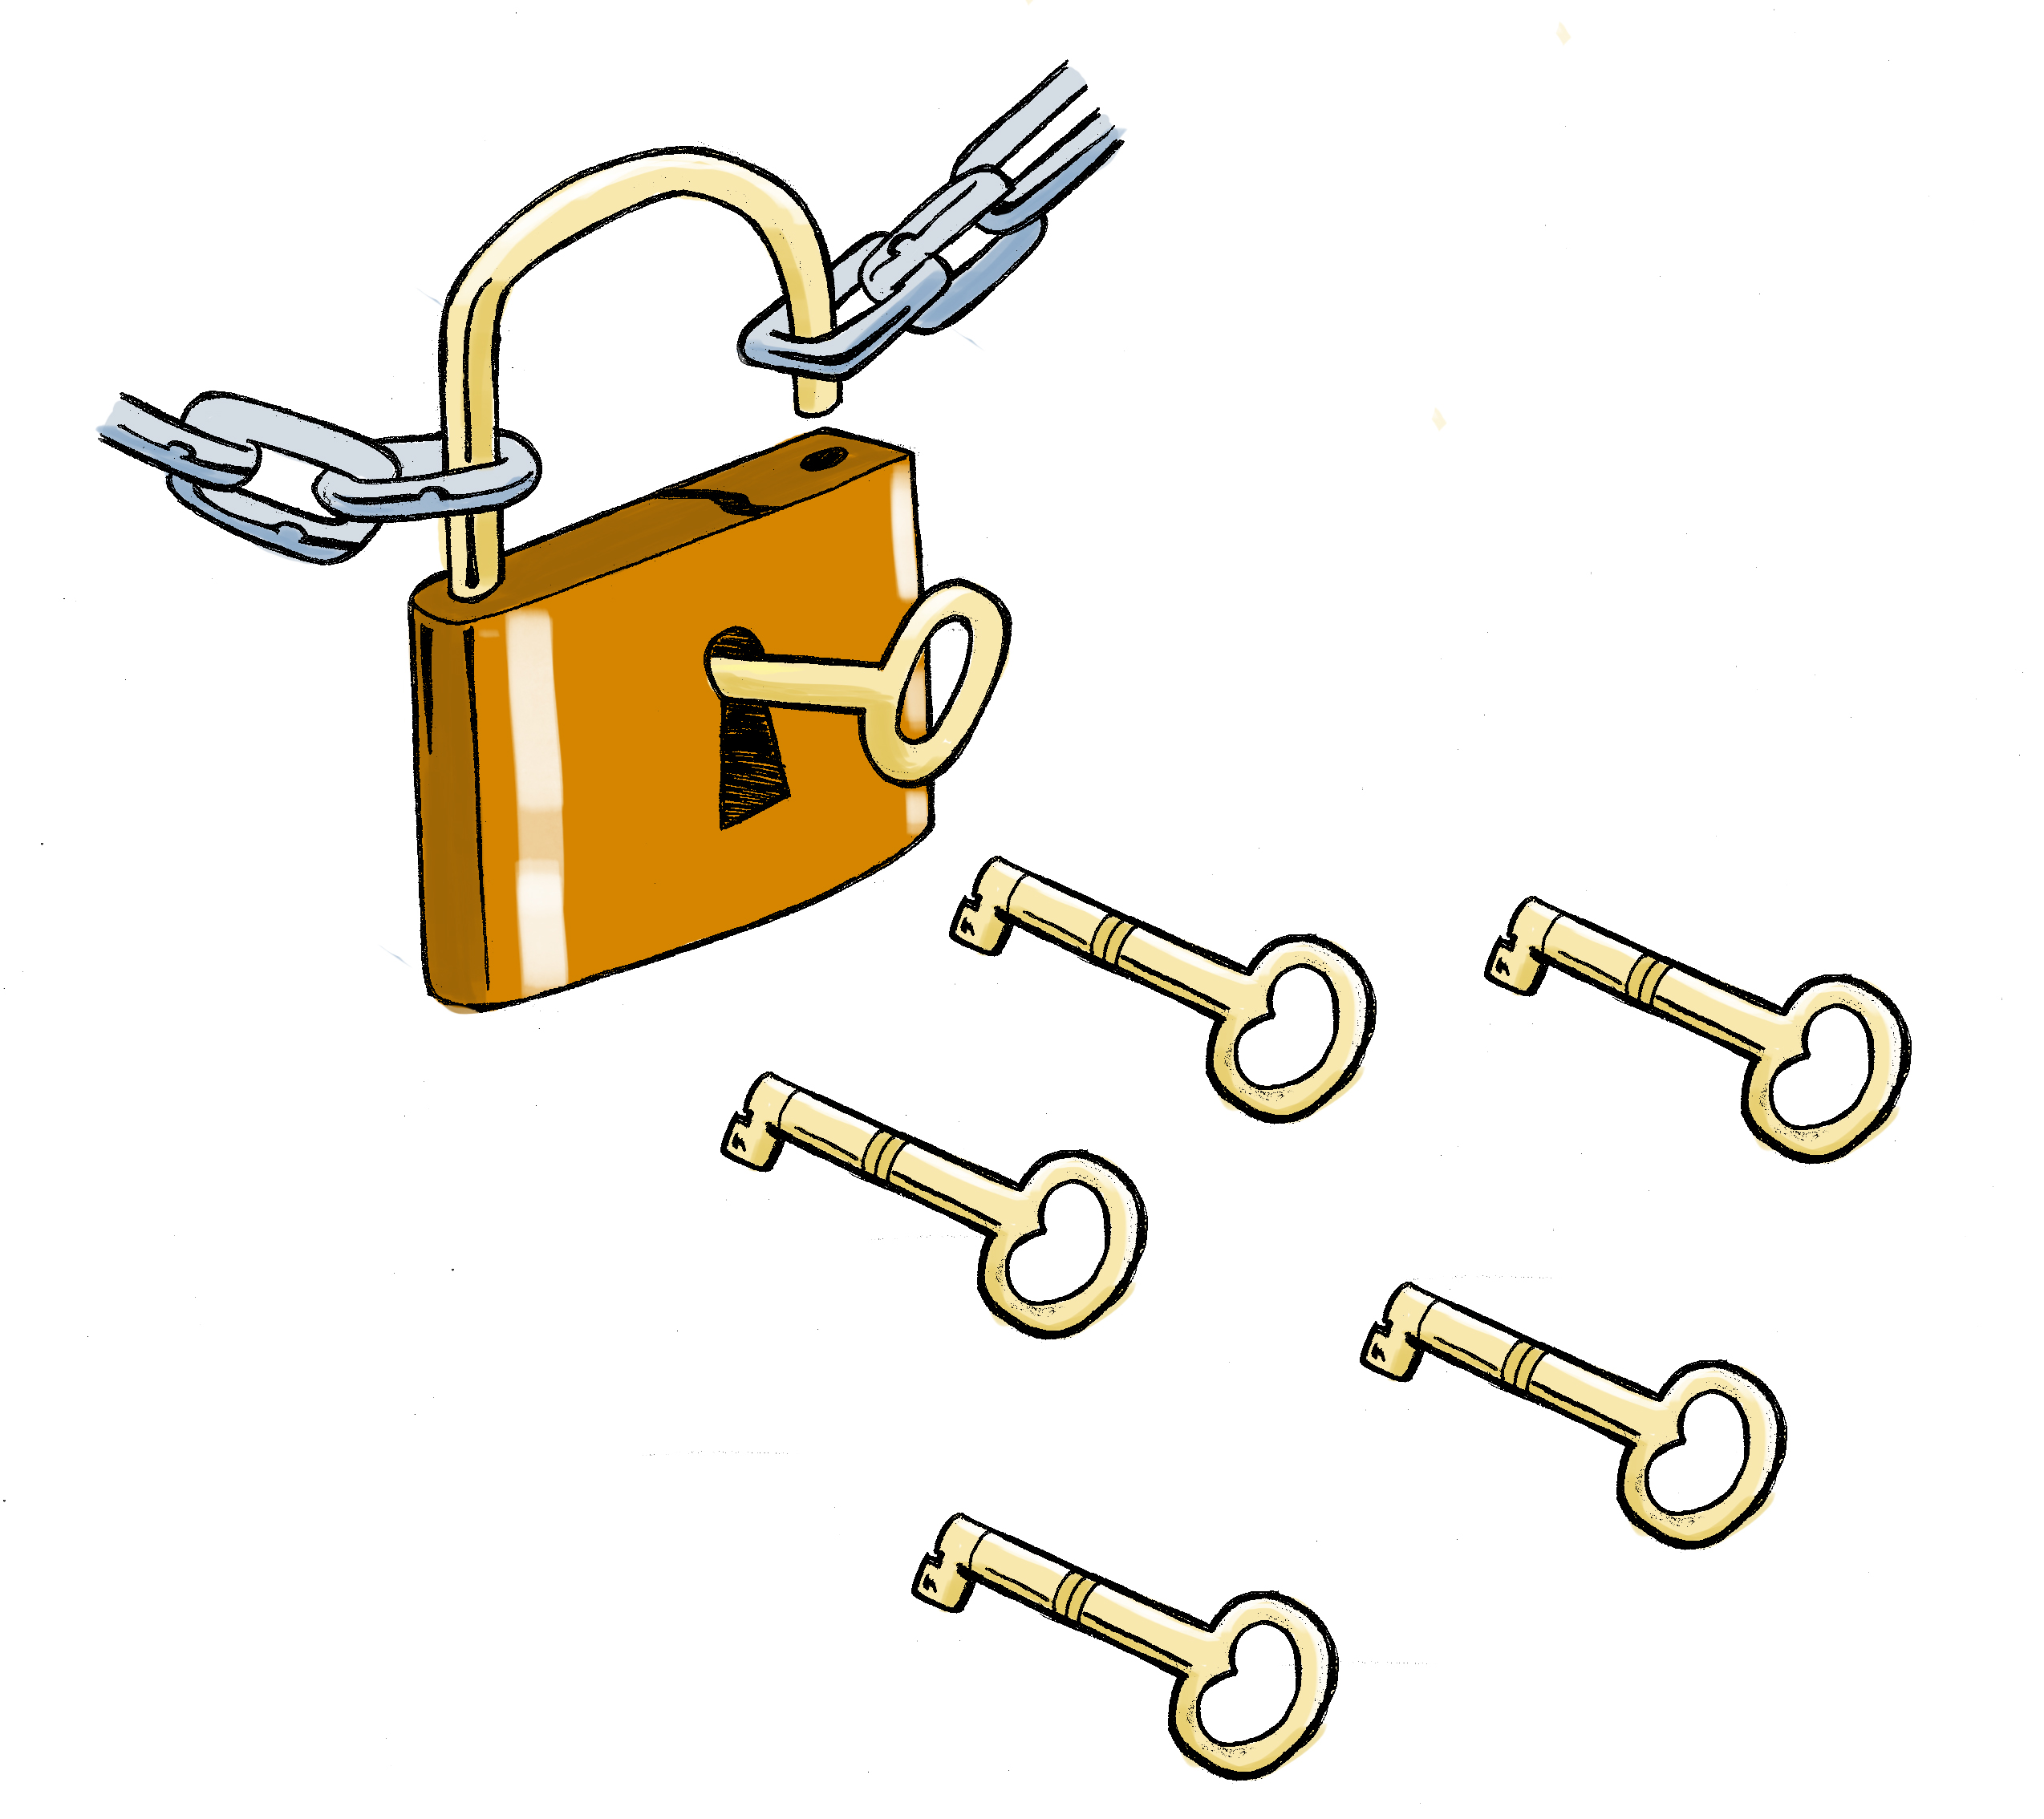
\includegraphics[width=175bp]{cadeado}

\caption{Chaves e cadeado}
\label{}
\end{figure}
Retirando-se chaves sequencialmente da caixa, qual a probabilidade de se abrir o cadeado apenas na terceira tentativa se:
\begin{enumerate}
\item a cada tentativa a chave extraída é recolocada na caixa?
\item a cada tentativa a chave extraída não é recolocada na caixa?
\item Em qual dos contextos (a) e (b) a probabilidade de se abrir a caixa é maior? Por quê?
\end{enumerate}

\ifdefined\prof
\begin{solucao}

\begin{enumerate}
\item Sejam os eventos $A_i$: “o cadeado é aberto na $i$-ésima tentativa”, $i=1,2,3$. Queremos calcular $P(\overline{A_1}\cap \overline{A_2}\cap A_3)$ , pois por hipótese o cadeado não foi aberto nem na primeira nem na segunda tentetiva.

$P(\overline{A_1}∩\overline{A_2}\cap A_3)=P(\overline{A_1})\cdot P(\overline{A_2}|\overline{A_1})\cdot P(A_3|\overline{A_1}\cap \overline{A_2})=\frac{4}{5}\cdot\frac{4}{5}\cdot\frac{1}{5}=\frac{16}{125}=0{,}128$. Essa solução pode ser visualizada por meio do diagrama de árvore, ilustrado na figura a seguir.
\begin{figure}[H]
\centering

\resizebox{.95\linewidth}{!}
{
\begin{tikzpicture}[every node/.style={scale=3}]
\draw (0,0) -- (30:3) node [right, scale=0.28] {$A_1$} node [above, midway, rotate=30, scale=0.28] {1/5};
\draw (0,0) -- (-30:3) node [right, scale=0.28] {$\overline{A_1}$} node [below, midway, rotate=-30, scale=0.28] {4/5};

\draw [->] (3.159807,1.5) -- ++(0:0.7) node [right, scale=0.28] {Abre na Primeira $\quad P(A_1) = \dfrac{1}{5}$} ;

\draw (3.159807,-1.5) -- ++(30:3) node [right, scale=0.28] {$A_2$} node [above, midway, rotate=20, scale=0.28] {1/5};
\draw (3.159807,-1.5) -- ++(-30:3) node [right, scale=0.28] {$\overline{A_2}$} node [below, midway, rotate=-20, scale=0.28] {1/5};

\draw [->] (6.319614,0) -- ++(0:0.7) node [right, scale=0.28] {Abre na Segunda $\quad P(A_1 \cap A_2) = \dfrac{4}{5} \cdot \dfrac{1}{5}$} ;


\draw (6.319614,-3) -- ++(30:3) node [right, scale=0.28] {$A_3$} node [above, midway, rotate=20, scale=0.28] {1/5};
\draw (6.319614,-3) -- ++(-30:3) node [right, scale=0.28] {$\overline{A_3}$} node [below, midway, rotate=-20, scale=0.28] {1/5};

\draw [->, align=left] (9.479421,-1.5) -- ++(0:0.28) node [ right, scale=0.28] {Abre na Segunda \\ $P(A_1 \cap A_2 \cap A_3) = \dfrac{4}{5} \cdot \dfrac{4}{5} \cdot \dfrac{1}{5}$} ;

\end{tikzpicture}
}
\item 
\end{figure}
\item Considerando agora o caso sem reposição tem-se
$P(\overline{A_1}\cap \overline{A_2}\cap A_3)=P(\overline{A_1})\cdot P(\overline{A_2}|\overline{A_1})\cdot P(A_3|\overline{A_1}\cap\overline{A_2})=\frac{4}{5}\cdot\frac{3}{4}\cdot\frac{1}{3}=\frac{1}{5}=0{,}2$. Essa solução pode ser visualizada por meio do diagrama de árvore, ilustrado na figura a seguir.

\begin{figure}[H]
\centering

\begin{tikzpicture}[every node/.style={scale=3}]

\draw (0,0) -- (30:3) node [right, scale=0.28] {$A_1$} node [above, midway, rotate=30, scale=0.28] {1/5};
\draw (0,0) -- (-30:3) node [right, scale=0.28] {$\overline{A_1}$} node [below, midway, rotate=-30, scale=0.28] {4/5};

\draw [->] (3.159807,1.5) -- ++(0:0.7) node [right,  scale=0.28] {Abre na Primeira $\quad P(A_1) = \dfrac{1}{5}$} ;

\draw (3.159807,-1.5) -- ++(30:3) node [right, scale=0.28] {$A_2$} node [above, midway, rotate=20, scale=0.28] {1/4};
\draw (3.159807,-1.5) -- ++(-30:3) node [right, scale=0.28] {$\overline{A_2}$} node [below, midway, rotate=-20, scale=0.28] {3/4};

\draw [->] (6.319614,0) -- ++(0:0.7) node [right, scale=0.28] {Abre na Segunda $\quad P(A_1 \cap A_2) = \dfrac{4}{5} \cdot \dfrac{3}{4}$} ;


\draw (6.319614,-3) -- ++(30:3) node [right, scale=0.28] {$A_3$} node [above, midway, rotate=20, scale=0.28] {1/3};
\draw (6.319614,-3) -- ++(-30:3) node [right, scale=0.28] {$\overline{A_3}$} node [below, midway, rotate=-20, scale=0.28] {2/3};

\draw [->, align=left] (9.479421,-1.5) -- ++(0:0.7) node [ right, scale=0.28] {Abre na Segunda \\ $P(A_1 \cap A_2 \cap A_3) = \dfrac{4}{5} \cdot \dfrac{3}{4} \cdot \dfrac{1}{3}$} ;
\end{tikzpicture}
\end{figure}
\end{enumerate}

\end{solucao}
\fi

\end{document}